\chapter{绪论}

\section{模式(字符串)匹配}

模式匹配(Pattern Matching, 简称PM), 一直以来都是计算机科学的核心问题之
一。 这里的“模式”特指字符串。 对于很多应用, 例如模式识
别 \cite{Yan2016}, \cite{Xiao2016}, 本体匹配 \cite{Xue2015}
\cite{Xue2016}, 文本分类 \cite{Tang2015} \cite{Zhang2016}, 系统安
全 \cite{Dien2014,Malhotra2016,Fan2016},入侵检测系
统 \cite{Kim2015,Arney2016,Sadotra2016,Lee2017} 等等, 模式匹配算法都是
最为基本而重要的操作。根据待匹配模式的数量,模式匹配技术可以分为两类:
单模式匹配(SPM)和多模式匹配(MPM)。

\begin{figure}[!h]
  \centering
  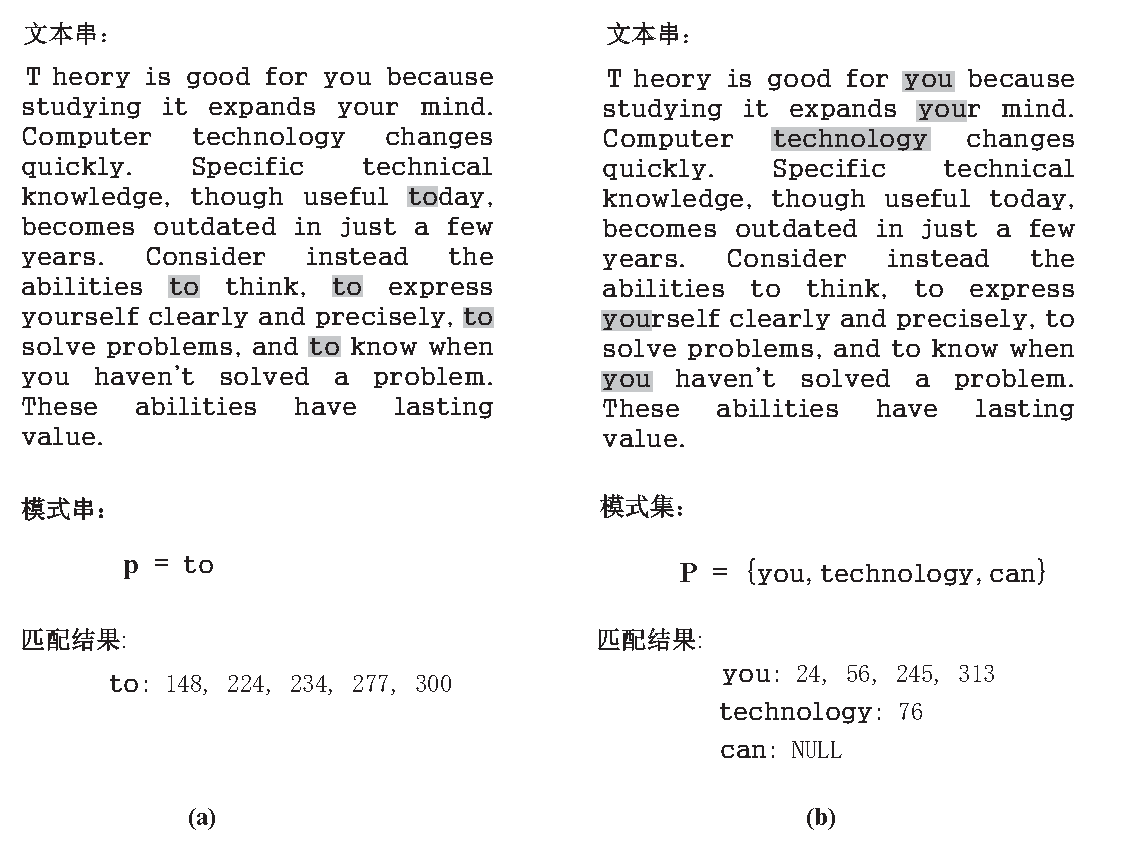
\includegraphics[height=8cm ,width=12cm]{figures/1_Introduction/SPM_MPM.eps}
  \caption{(A) 单模式匹配示例。(B) 多模式匹配示例。}
  \label{fig:SPM_MPM}
\end{figure}


\subsection{单模式匹配}

单模式匹配算法要求在文本串中寻找给定模式串的所有出现位置。如
图 \ref{fig:SPM_MPM } (A) 所示, 给定文本串与模式$to$, 经过匹配发现,模
式串$to$ 出现于文本串中的位置为: 148, 224, 234, 277, 300。

最简单的单模式匹配算法,需要对文本串中的每一个位置与模式串进行逐字符的
比较,一旦出现字符失配,将直接移动到文本串的下一个位置进行匹配。很明显,
当文本串的长度为$n$且模式串的长度为$m$时,这种简单的模式匹配算法的时间
复杂度为$O(m \cdot
n)$。当文本串形如$aaa \dots
a$及模式串为$aaab$时,将出现最坏情况。为此,有更加高效的单模式匹配算法
被提出,最著名的包括KMP \cite{Knuth1977}算法 和 BM \cite{Boyer1977} 算
法。下面将简单介绍这两种算法的核心思想。

1. \textbf{KMP(Knuth-Morris-Pratt)算法}

KMP算法的核心思想在于,一旦匹配失败,可以充分利用已经匹成功的子串信息,
让模式串向右移动尽可能多的位置。右移的距离是这样计算的:在已经匹配的模
式串子串中,找出最长的相同的前缀和后缀,然后向右移动使它们重叠。如
图\ref{fig:KMP}(A)所示,在当前匹配中,文本串中的位置10($i=10$)和模式串
中的位置8($j=8$)出现失配,根据已经匹配成功的子串即$abcdaabc$的信息:该
子串相等的最长前缀与最长后缀是$abc$, 将模式串向右移动使得这两部分相重合,
如图 \ref{fig:KMP} (B)
所示。此时,文本串中当前待匹配位置$i$不变,而模式串中当前待匹配位
置$j$变为3,分别从位置$i$和$j$开始对文本串和模式串进行逐字符比较。KMP算
法在匹配过程中,文本串中的当前匹配位置$i$永不减小,只是当匹配失败时,根
据模式串中的失配位置,来调整模式串中的下一次与文本串位置$i$相比较的位置。
因此,需要知道在失配时,下一次应当用模式串的哪个位置与文本串进行比较。
为此对模式串进行预处理,为其建立失配数组$Next$(如图 \ref{fig:KMP} (C)所
示),
如果当前在模式串的位置$j$失配时,下一次将用模式串的位置$Next[j]$来与文
本串进行比较,预处理过程的时间复杂度为$O(m)$($m$为模式串长度)。 由于匹
配过程中, 文本串中的位置$i$永不回溯,所以KMP算法的时间复杂度为$O(m+n)$
($n$为文本串长度)。

\begin{figure}[!h]
  \centering
  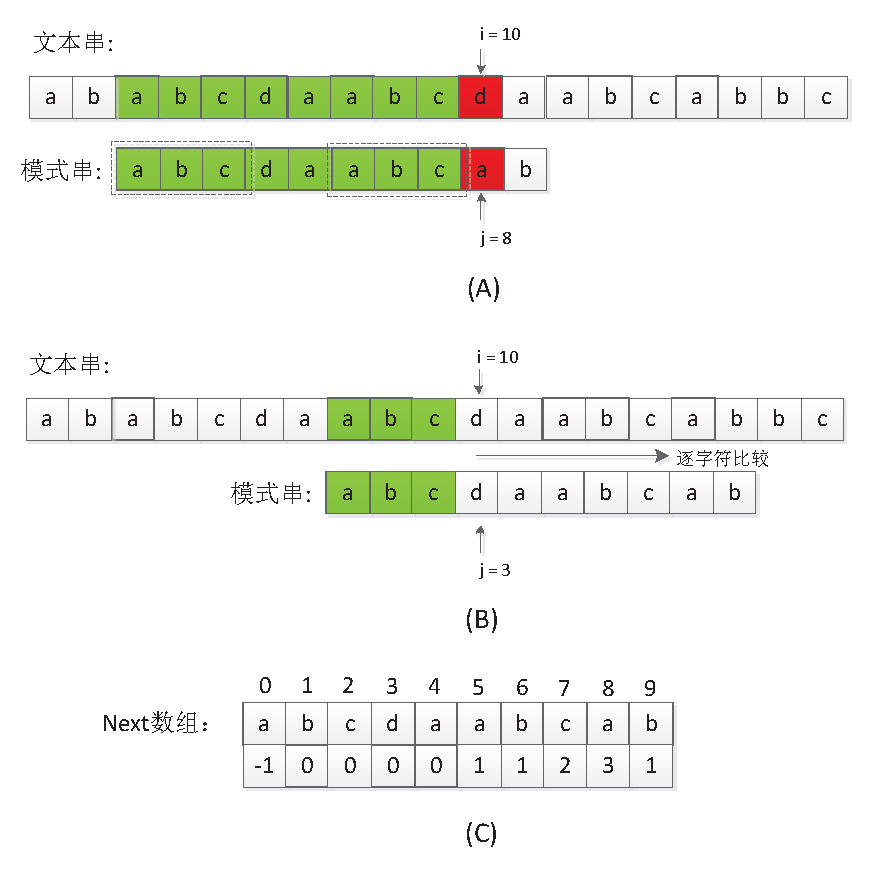
\includegraphics[height=10cm ,width=12cm]{figures/1_Introduction/KMP.eps}
  \caption{KMP算法示例。(A) 第一轮匹配。(B) 第二轮匹配。(C) 模式串
    的Next数组。}
  \label{fig:KMP}
\end{figure}


2. \textbf{BM(Boyer-Moore)算法}

尽管KMP算法具有线性的时间复杂度,可其实际的速度却并不快。在实际应用当中
(比如各类字处理软件中的字符串查找功能),最常用的单模式匹配算法是BM算
法 \cite{Boyer1977}, 及其诸多变体。BM算法最高效之处在于通过使用“坏字
符”规则,其可以快速跳过文本串中大量的不可能出现匹配的位置。如
图 \ref{fig:BM} (A) 所示,BM算法采用从右到左的方向对模式串与文本串进行
比较,由于第一次比较即失配且文本串中相应的字符$s$没有出现在模式串中,因
此可以将模式串整体向右移动到$s$的下一个字符处,然后再别从位
置13($i=13$)和位置6($j=6$),从右向左地对文本串和模式串进行比较,如
图 \ref{fig:BM} (B)
所示。由于再次失配,且文本串中的字符$p$出现于模式串中,因此将模式串向右
移动2个位置,使两个串中的$p$字符对齐,如图\ref{fig:BM}(C)所示。由于BM算
法在每次匹配失败时,都将根据文本串中的失配字符来移动模式串,因此需要对
整个字符集进行预处理构建坏字符表(表长为$|\Sigma|$,即字符集大小),当
匹配失败时用文本串中的失配字符作为索引来查找坏字符表,来决定需要将模式
串向后移动多少位。BM算法最坏情况的时间复杂度为$O(n \cdot m)$,但是在实
际中很少出现这样的情况。

\begin{figure}[!h]
  \centering
  \includegraphics[height=10cm ,width=12cm]{figures/1_Introduction/BM.eps}
  \caption{BM算法示例。(A) 第一轮匹配。(B) 第二轮匹配。(C) 第三轮匹配。}
  \label{fig:KMP}
\end{figure}

\subsection{多模式匹配}

多模式匹配要求找出给定模式集中每一个模式串在文本串中的所有出现位置。如
图 \ref{fig:SPM_MPM} (B) 所示,给定模式集
$P={can, you, technology}$及文本串,通过多模式匹配发现, 模式串$you$出现
了4次, 模式串$technology$出现了1次, 模式串$can$在文本串中没有出现。

目前,多模式匹配算法的主要流程是先对模式集进行预处理,构建合适的数据结
构来存储和组织模式集中的模式串,然后用构建好的数据结构和文本进行比较,
一次性找出所有模式集的出现位置。 比较著名的多模式匹配算法包括 AC
\cite{Aho1975} 和 WM \cite{Wu1994} 算法。

1. \textbf{AC(Aho-Corasick)算法}

AC算法是经典的多模式匹配算法,它是KMP算法在多模式环境下的推广,具有线性
时间复杂度。目前,各种AC算法的变体在实际当中被广泛应用。AC算法通过为模
式集构造一个有限状态自动机(DFA),然后将文本串中的每一个字符输入到自动机
中进行状态转移,来实现多模式匹配。图 \ref{fig:AC} 所示的是为模式
集$P=\{he, his, she, hers\}$ 所构造的AC自动机,图中实线箭头及对应字符表
示,在当前状态遇到该字符时应该跳转到的状态,虚线表示在当前状态无匹配字
符时,应该跳转到的状态,图中绿色的状态,表示匹配成功状态。 匹配时,AC算
法将从状态0开始,连续不断地读入文本串中的字符,并根据所读入的字符进行状
态跳转,一旦到达匹配成功状态,将输出匹配到的模式串。 举例说明,假设文本
串为$hers$, 初始状态为0, 第一个文本串字符为$h$, 则自动机将跳转到状态1;
下一个输入字符为$e$,
将跳转到状态2,同时成功匹配模式串$he$并将其输出;下一个字符为$r$,将跳
转到状态8;最后一个字符为$s$,跳转到状态9,并输入匹配成功的模式
串$hers$。传统的AC算法对字符集大小非常敏感,对于较大的字符集,算法所构
造的自动机将会消耗大量的空间,且在实际应用中性能较低。


\begin{figure}[!h]
  \centering
  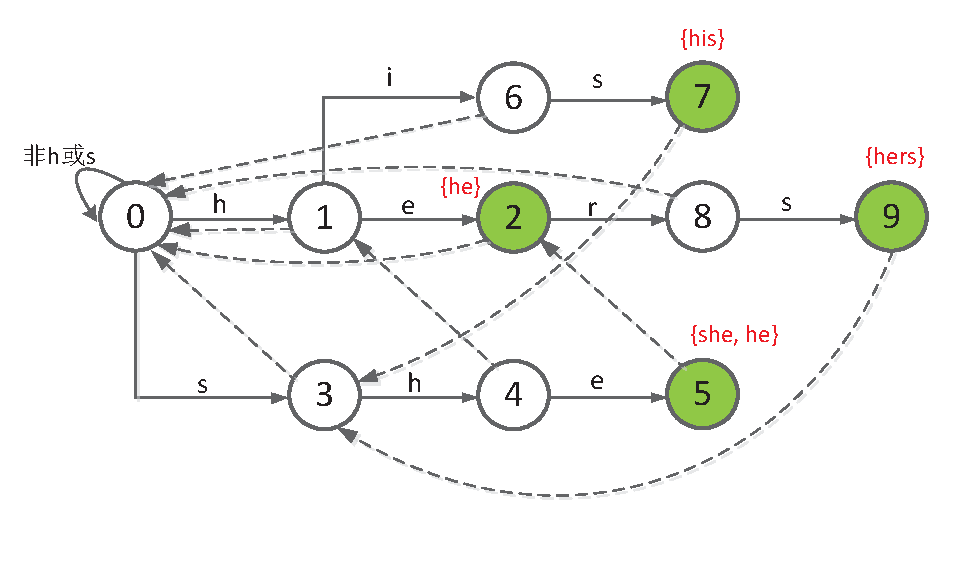
\includegraphics[height=7cm ,width=10cm]{figures/1_Introduction/AC.eps}
  \caption{为模式集$P=\{he, his, she, hers\}$所构建的AC自动机。}
  \label{fig:AC}
\end{figure}

2. \textbf{WM(Wu-Manber)算法}

 WM算法是BM算法在多模式环境下的推广,BM算法采用“坏字符”规则在文本中
进行跳跃,而由于模式串个数的增加,WM算法将采用“坏字符块”技术,增大了
文本串和模式串不匹配的可能性.从而增加了直接跳跃的机会。它还使用前缀表
进一步过滤不匹配的模式串,使算法获得了较高的运行效率。

在预处理时,算法会为模式集构建3个表结构:哈希表,跳转表和前缀表。 跳转
表用于在扫描文本串的时候,根据读入字符串决定可以跳过的字符数,如果相应的
跳跃值为0,则说明可能产生匹配,就要使用哈希表和前缀表进一步判断, 以决定有
哪些匹配候选模式, 并验证究竟是哪个或者哪些候选模式完全匹配。因此,在现
有的多模式匹配算法中,使用块字符、哈希技术和前缀特征表技术的WM算法通常
被认为具有较高的效率,在实际中被广泛使用。 对WM更加具体的阐述将在第6章
介绍WM的改进算法时一并介绍。

\section{后缀数组}

后缀数组(Suffix Array, 简称SA)是由给定字符串的所有后缀按照字典序排列所
构成的数组,它是后缀树数据结构的空间高效的代替品,广泛地应用于全文索
引 \cite{Strate2015,Fischer2017,Arroyuelo2014},数据压
缩\cite{Louza2015,Chien2015,Pradhan2016,Brisaboa2015} 等领
域。 图\ref{fig:suffix}
中分别显示了为字符串$bananas$所构建的后缀树以及后缀数组。由于在给定字符
串之后,每个后缀便可由其起始位置完全确定,所以后缀数组中只需保留后缀的
起始位置,相比于后缀树,能够极大的节省存储空间。 并且,通过后缀树能完成
的一些文本操作,同样可以通过后缀数组(及一些辅助结构)等价地完成。

\begin{figure}[!h]
  \centering
  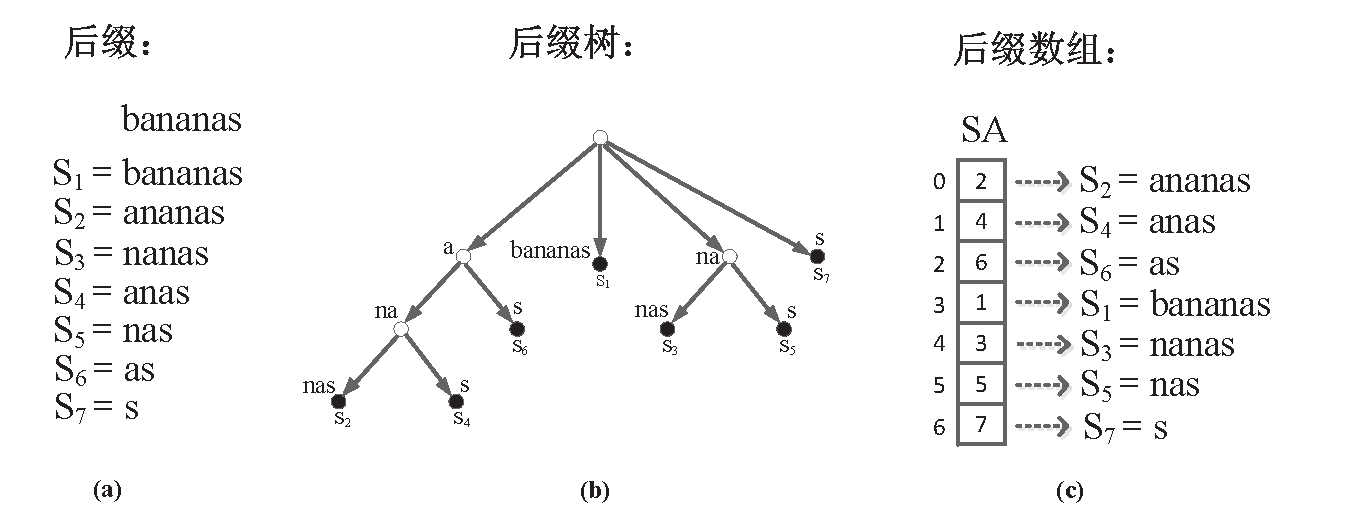
\includegraphics[height=7cm ,width=15cm]{figures/1_Introduction/Suffix.eps}
  \caption{(A) 字符串及其后缀。(B) 对应的后缀树。(C) 对应的后缀数组}
  \label{fig:Suffix}
\end{figure}

例如上一节中提到的单模式匹配问题,若模式串出现于文本串中,它必定是某
个(些)后缀的前缀,因此可以预先为文本串建立后缀树/数组,然后通过在后缀
树/数组上来查找模式串,可以在$O(m)$($m$为模式串长)时间内完成查找。举例
来说,假设文本串为$bananas$, 模式串为$an$, 对于后缀树,可以从其根节点开
始,对模式串进行逐字符遍历,之后发现有两个后缀即$S_3$与$S_5$都以$an$为
前缀,因此模式串$an$出现于文本串的第3和第5个位置。对于后缀数组,可以通
过在后缀数组上进行基于字典序的二分查找,同样可以快速地完成对模式串的搜
索。因此对那些不经常发生变化,且需要频繁进行查询操作的文本,可以预先为
其建立后缀数组,以加快查询速度。

很明显,构建后缀数组的过程实际上就是对后缀排序的过程。对后缀进行排序,
最直接的方法就是先对字符串构造后缀树,然后根据字符大小顺序深度优先遍历
后缀树,根据遍历到叶子节点的顺序来确定后缀的顺序。由于构造后缀树具有线
性时间复杂度的算法,因此理论上可以在线性时间内构造后缀数组。 然而,这种
方法不仅需要大量的存储空间,而且在实际中极其耗时。为此,应当研究直接对
后缀进行排序的方法,而非间接地通过后缀树来排序。

前缀倍增技术是实际应用当中广泛采用的后缀排序技术。其主要思想是由后缀的
首字符开始,逐步的来确定后缀之间的顺序,在第$k$轮中可以根据前$2^k$个字
符来对后缀进行排序,因此对长为$n$的字符串,最多需要$logn$轮,即可完成排
序十分的高效。举例来说,假设需要对字符串$bananas$的后缀进行排序。首先,
根据首字符对后缀进行排序,可将所有后缀分为4组,如
图\ref{fig:Prefix_Doubling}(A)所示。其中,组间有序而组内无序,即第1组中
的$S_6$, $S_4$,
$S_2$由于其首字符相同,此时还无法确定顺序,类似地,第3组中
的$S_5$和$S_3$也暂时无法确定顺序。由于$S_6$, $S_4$,
$S_2$首字符相同,因此它们之间的顺序取决于后面的字符串即$s$, $nas$,
$nanas$之间的顺序,这恰好是$S_7$, $S_5$,
$S_3$,由于$S_7$是字典序最大的后缀,所以$S_6$将大于$S_4$与$S_2$,又由
于$S_5$,
$S_3$次序待定,所以$S_4$与$S_2$次序待定。类似地,对于第3组中
的$S_5$和$S_3$,其顺序将由$S_6$与$S_4$决定,由于$S_6$大于$S_4$,$S_5$将
大于$S_3$,如图\ref{fig:Prefix_Doubling}(B)所示。最后,
第1组中$S_4$和$S_2$的顺序将取决于$S_6$和$S_4$, 由于$S_6$大于$S_4$,因
此,$S_4 $大于$S_2$,如图\ref{fig:Prefix_Doubling}(C)所示,排序完成。

\begin{figure}[!h]
  \centering
  \includegraphics[height=6cm ,width=15cm]{figures/1_Introduction/Prefix_Doubling.eps}
  \caption{利用前缀倍增技术对$bananas$的后缀进行排序。(A) 第一轮。(B) 第二轮。(C) 第三轮。}
  \label{fig:Prefix_Doubling}
\end{figure}
